subtasks are indicated by comments,
pure coding tasks are not listed
search for [some to include results


todo:
%I think it can be sensible to discuss the results as we are presenting them.
%A good strategy can be to move back to revise the introduction and think about what questions we want
%to ask (what are we actually answering?) and have this in mind as we  move on to the conclusion.


%problem 8
We simulate the motion of a particle in the Penning trap for $50 \mu s$ with initial conditions
\begin{align}
  (x_0, y_0, z_0) =& (20, 0, 20)\mu m, \\
  (u_0, v_0, w_0) =& (0, 25, 0) \mu m / \mu s.
\end{align}

%8.1

\begin{figure}
\centering
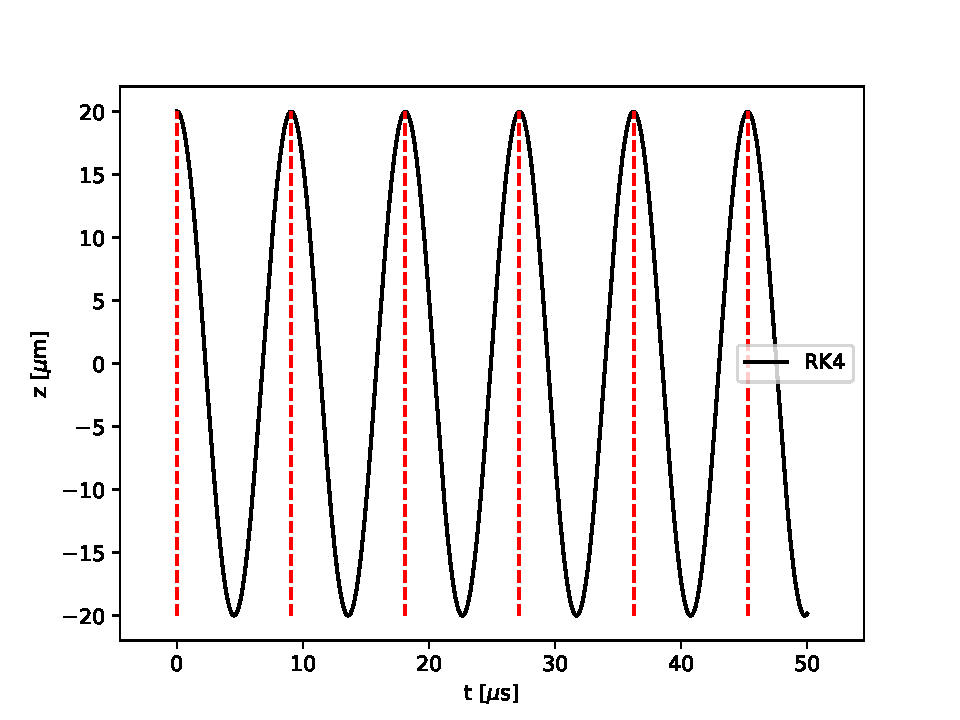
\includegraphics[scale = 1]{../figures/z_t_.pdf}
\caption{The motion of a single particle in the z-direction simulated for 50 $\mu$s. The dashed lines indicate the expected period of $T \approx 9$ $\mu$s.}
\label{fig:z_t_8}
\end{figure}

We show the motion of the particle in the $z$-direction over time in \autoref{fig:z_t_8}
The solution is a harmonic oscillator, as seen from \autoref{eq:eom_z}. The dashed lines in the figure indicate the anticipated period of $T = \frac{2\pi}{\omega_z} \approx 9$ $\mu$s.

%8.5 and 8.6
\begin{figure}
\centering
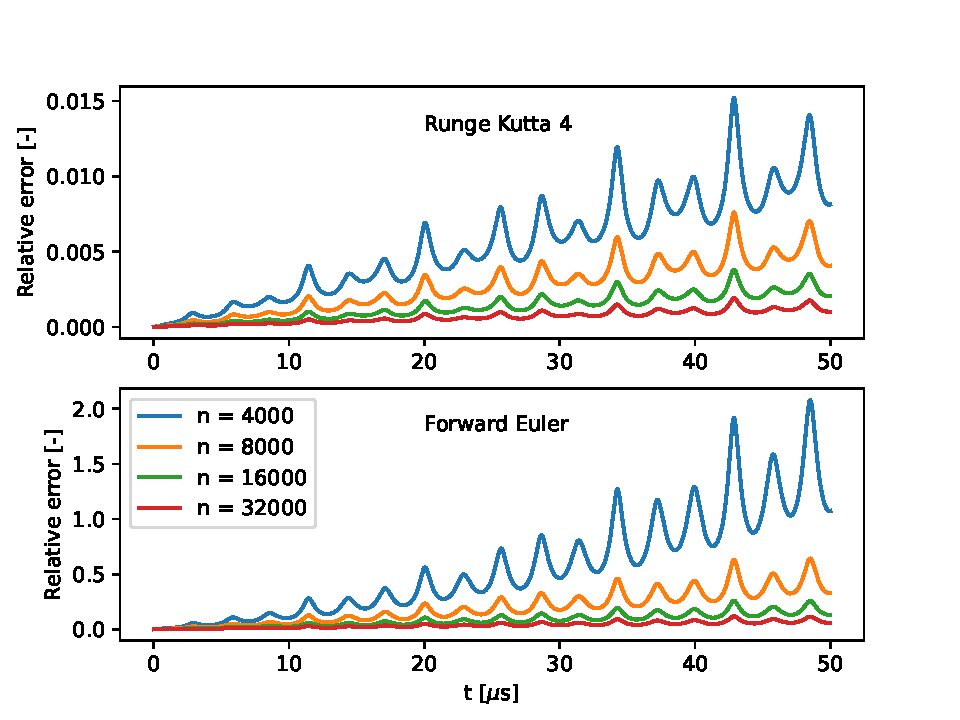
\includegraphics[scale = 1]{../figures/convergence.pdf}
\caption{}
\label{fig:converge}
\end{figure}

We simulate decreasing time steps to test the convergence of FE and RK4.
We divide our domain into $4000$ and double the number of steps consecutively three times,
resulting in four simulations with decreasing time steps. The results are in \autoref{fig:converge}.
%%%%%%%%%%%%%%
We see from this plot that the relative error in the RK4 solution is roughly two orders of magnitude lower
than that of the FE solution. However, the rate of convergence is higher for FE than for
RK4. This is also confirmed by the convergence rate, which is $r_{\text{RK4}} \approx 1$ and $r_{\text{FE}} \approx 1.4$. 
The formula used to calculate the convergence rate is shown in \autoref{sec:app}. Since the global error of FE is $h$ and RK4 is $h^2$
We expect to see the RK4 algorithm converge faster as the time step decreases. However, this is not the case, and we think that it can 
be since our RK4 algorithm is already good enough with smaller time step, as the Forward-Euler algorithm, as discussed just below,
perform poorly with bigger time step. 

\begin{figure}
\centering
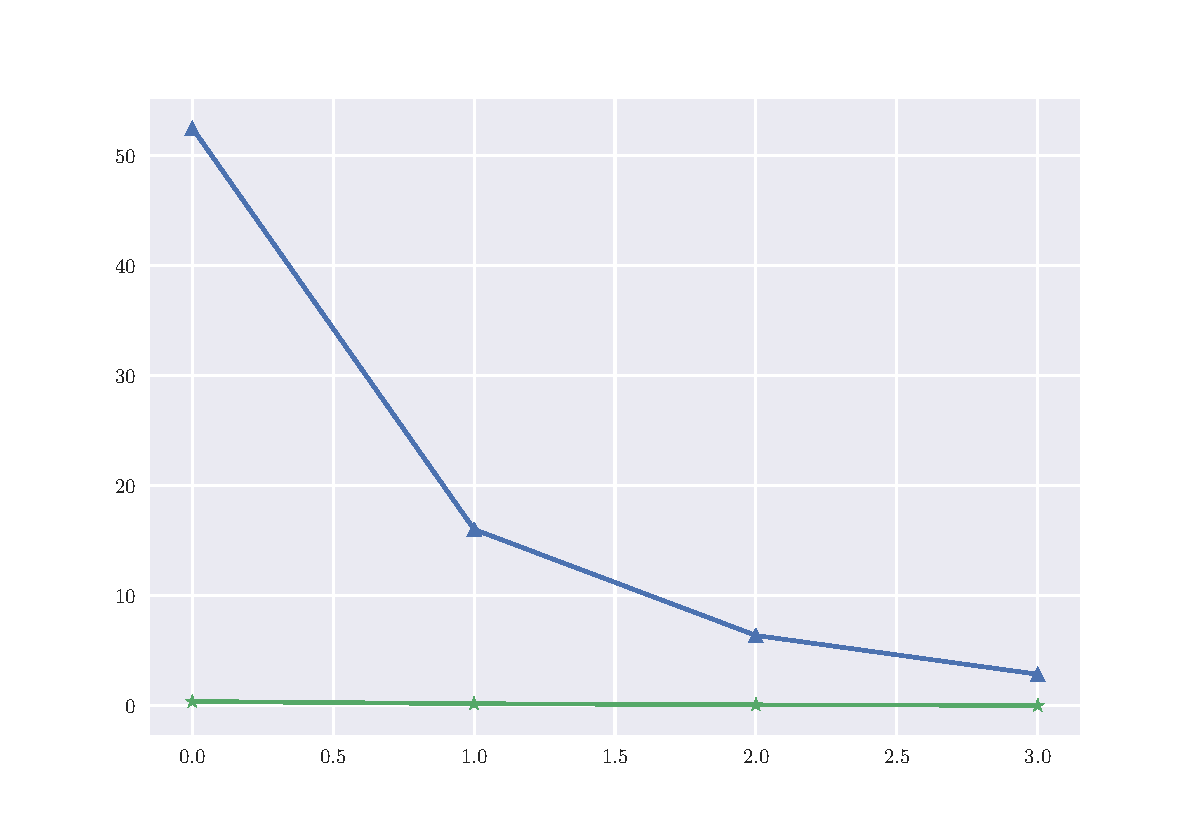
\includegraphics[scale = 1]{../figures/del_max.pdf}
\caption{}
\label{fig:del_max}
\end{figure}

We can see that the Forward-Euler algorithm could be more accurate than the Runge-Kutta fourth-order algorithm. This is to be
expected, but the error is more significant than we would expect, as seen in \autoref{fig:del_max}. Also, we observe that the error does not diminish 
as much as expected since the error is proportional to $dt^2$. From this, we can think there is still some small error in the code but
not big enough to discard any results. 




%8.2 and 8.4
To look at the effect of the Coulomb interaction, we add another particle to the mix with the initial
conditions
\begin{align}
  (x_0, y_0, z_0) =& (25, 25, 0)\mu m, \\
  (u_0, v_0, w_0) =& (0, 40, 5) \mu m / \mu s.
\end{align}

\begin{figure}
\centering
\includegraphics[scale = 0.7]{../figures/3d_noint.pdf}
\includegraphics[scale = 0.7]{../figures/3d_int.pdf}
\caption{3D plots of the particle trajectories with and without interactions. The trajectory of Particle 1 is shown in blue, whereas the trajectory of Particle 2 is orange. }
\label{fig:3d}
\end{figure}

\begin{figure}
\centering
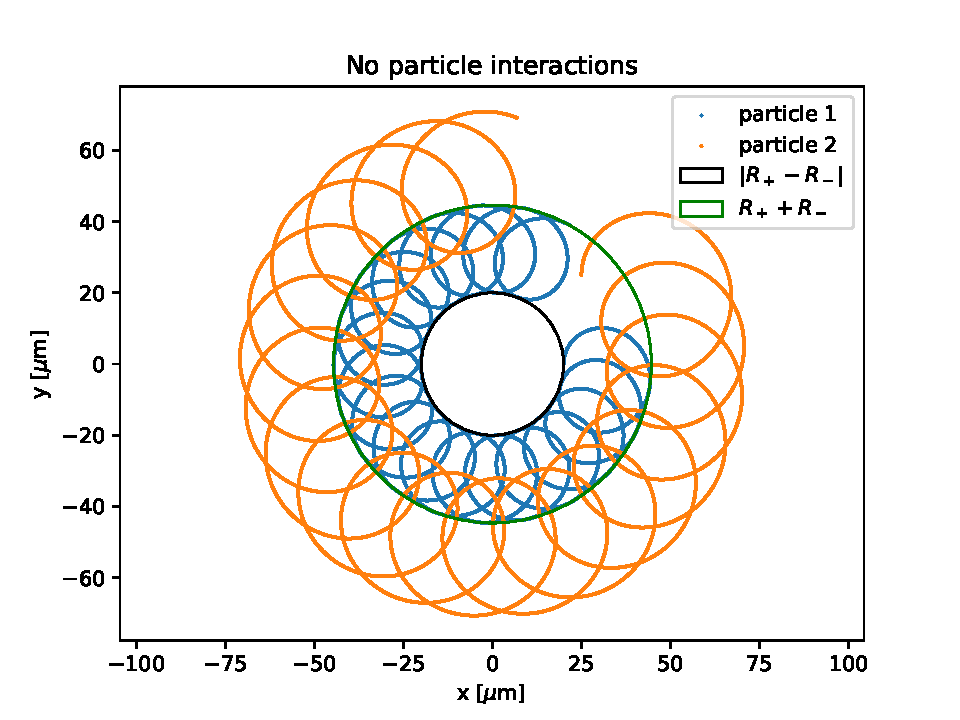
\includegraphics[scale=0.7]{../figures/xy_plane_noint.pdf}
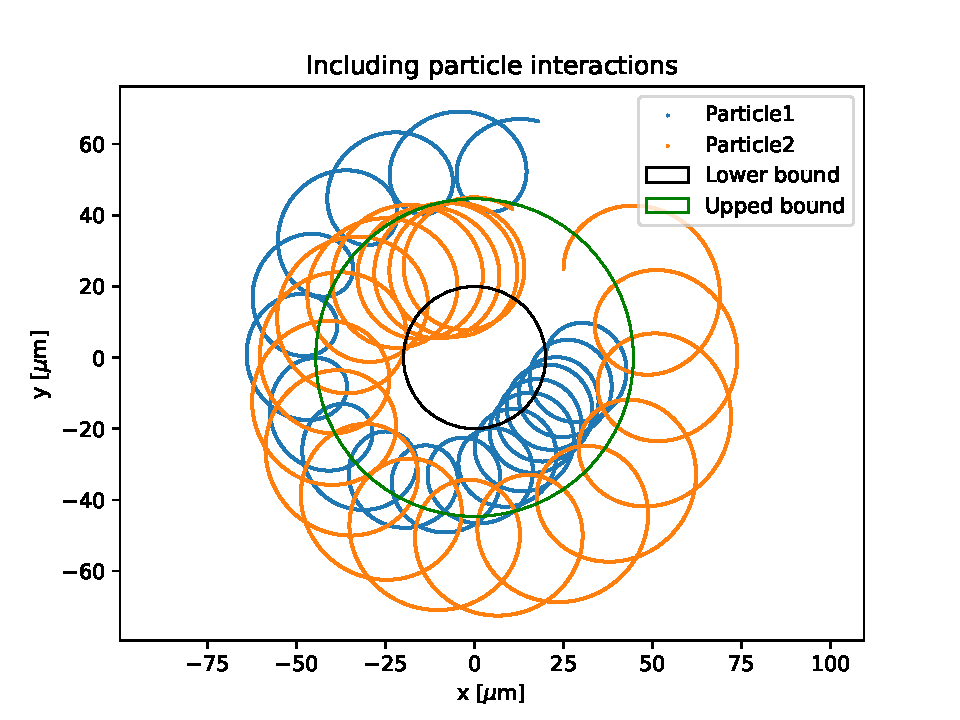
\includegraphics[scale=0.7]{../figures/xy_plane_int.pdf}
\caption{Plot of Particle 1 (blue) and Particle 2 (orange) with and without
the effects from the Coulomb interactions. The simulations start in the right half of the
figure, and the particles 'orbit' clockwise about the trap's centre. The upper and lower bounds on Particle 1's analytical solutions are displayed as green and black circles.} %
\label{fig:xy_plane}
\end{figure}

\begin{figure}
\centering
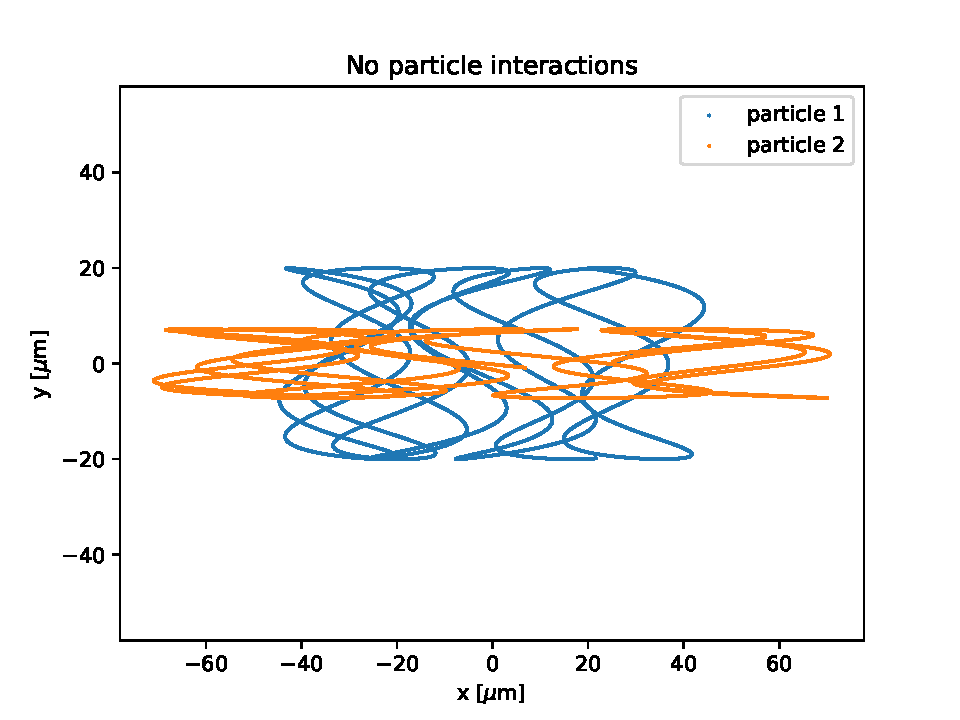
\includegraphics[scale=0.7]{../figures/xz_plane_noint.pdf}
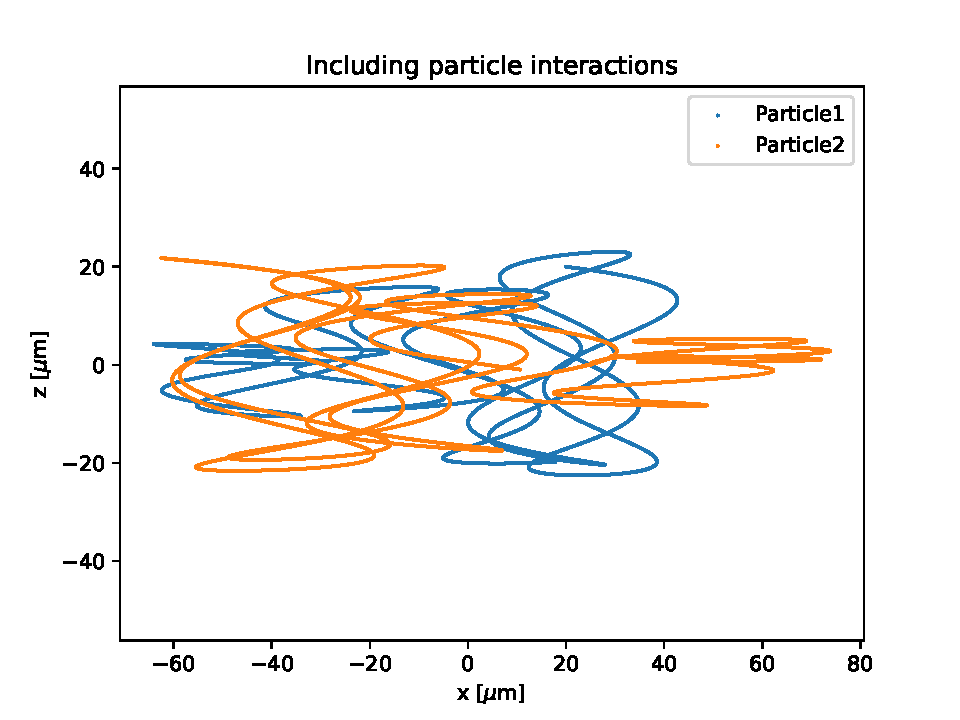
\includegraphics[scale=0.7]{../figures/xz_plane_int.pdf}
\caption{Particle 1 (blue) and Particle 2 (orange) with and without taking into account Coulomb interactions.}
\label{fig:xz_plane}
\end{figure}

The trajectories of the particles are shown in \autoref{fig:3d}, both calculating with interactions and
neglecting interactions. To better understand the effects of the interactions. We look at two
different projections of the trajectories, onto the $xz$-plane and the $xy$-plane.

The particle trajectories in the $xz$-plane are shown in \autoref{fig:xz_plane}. When we include interaction, the particles span a larger region in the $z$-direction, as expected. Since the particles
are repulsive, they tend to be far apart. A similar effect can be seen
in the $xy$-plane, \autoref{fig:xy_plane}. Here we can tell that the presence of Particle 2
pushes Particle 1 beyond the bounds of its analytical solution. At first, it looks as if Particle 1
is being squashed in towards the centre. Then they swap places, and Particle 1 is on the outside and the
Particle 2 seems to have a compressed trajectory with denser precessions.

%8.3
\begin{figure}
\centering
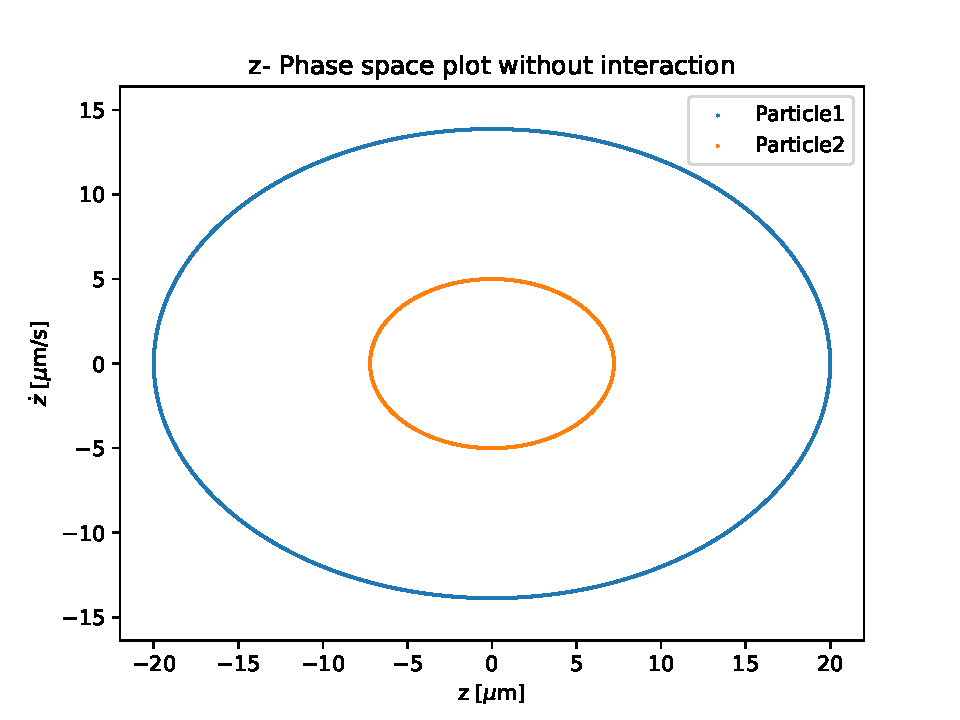
\includegraphics[scale = 0.7]{../figures/z_phase_noint.pdf}
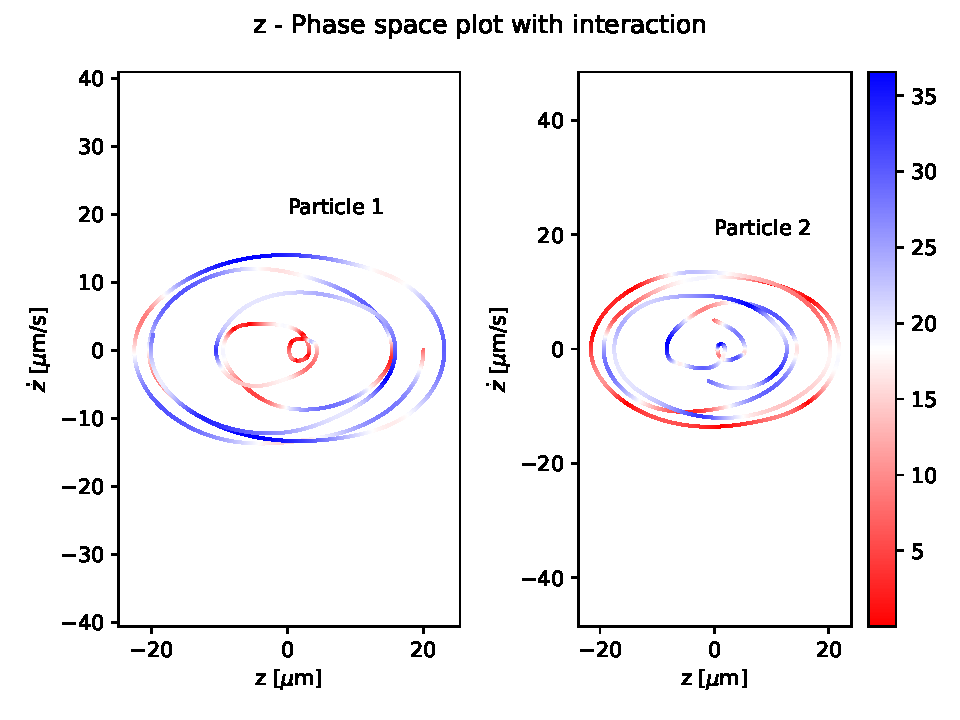
\includegraphics[scale = 0.7]{../figures/z_phase_int.pdf}
\caption{Phase space trajectories (z, w) of Particle 1 and Particle 2. Above, Particle 1 is blue, and Particle 2 is orange.
The simulations for the topmost plot were run neglecting Coulomb interactions. The bottommost simulation includes Coulomb interactions. In the bottom figure, we draw the particle trajectories in
separate plots for clarity, the colour indicates the distance between the particles. The colour bar scale is
$\mu$m.}
\label{fig:phase_z}
\end{figure}

\begin{figure}
\centering
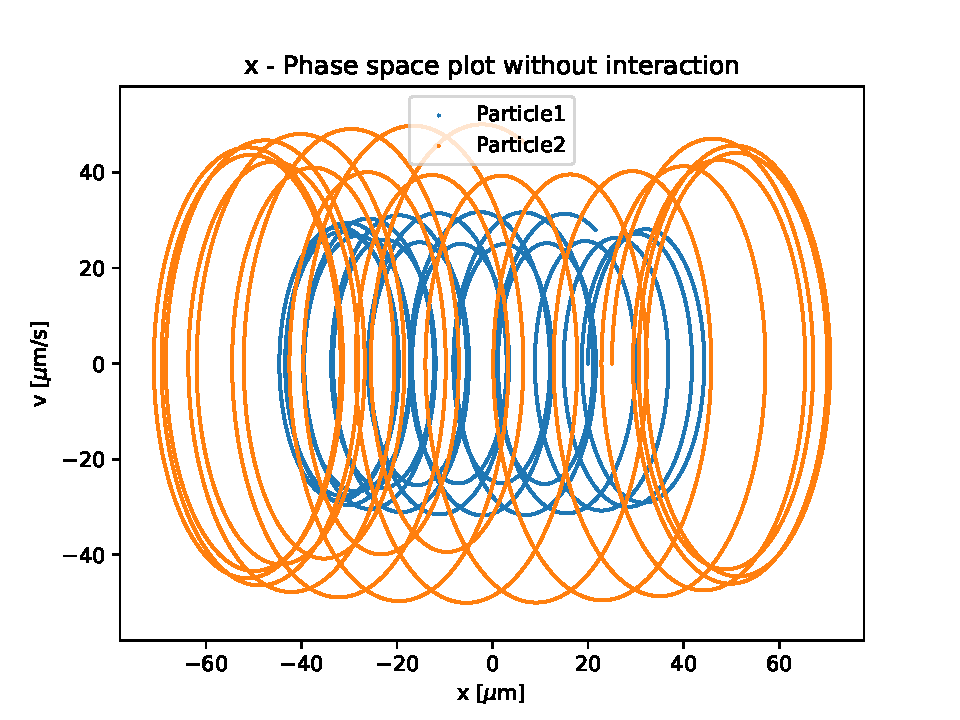
\includegraphics[scale = 0.7]{../figures/x_phase_noint.pdf}
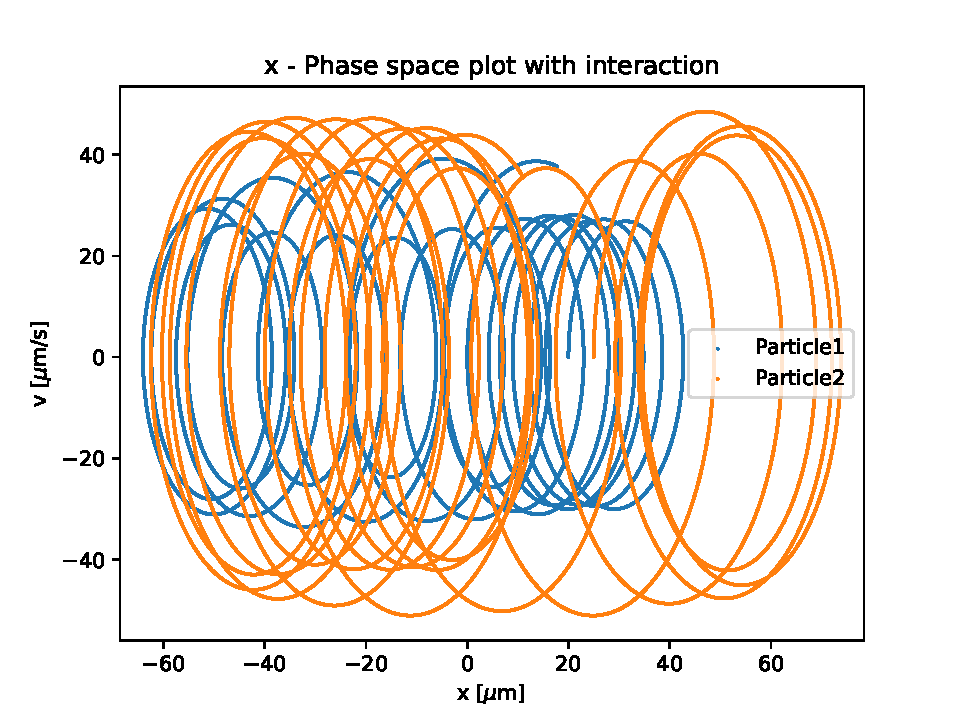
\includegraphics[scale = 0.7]{../figures/x_phase_int.pdf}
\caption{Phase space plots of Particle 1 (blue) and Particle 2 (orange), the trajectories look a bit like cylinders,
we expect them to encircle a torus in 3D.
When we include Coulomb interactions, the trajectories get distorted compared to the idealized case.}
\label{fig:phase_x}
\end{figure}


We see a plot of the particles' motion in phase space along the $z$-axis in \autoref{fig:phase_z}. Without particle interactions, the phase space trajectories are
elliptic. The energy of each particle is conserved and transitions back and forth
between kinetic and potential energy.

When the Coulomb interactions are included, the particles can exchange energy. This makes it possible for both particles to lose or gain energy, making
a larger region of phase space available for them.
The potential energy of one particle, due to the presence of the other particle, is indicated by the colour of the trajectory. Red indicates high energy, and blue indicates low energy. Notice that at
a portion of the trajectories where the particles are close, Particle 1 is generally closer to the
origin, implying it has lower energy. In contrast, Particle 2 is further from the origin, implying it has higher potential or kinetic energy. The interactions between the particles allow them to swap places
in phase space.

In the phase space projected onto the $x$-direction, \autoref{fig:phase_x}, the phase space plots look more complicated.
We, for example, recognize the precessions also seen in \autoref{fig:xy_plane}, the particle frequently changes direction, that is
crosses $v=0$ in the figure.
The the equation of motion for a particle in the x-direction \autoref{eq:eom_x} has three variables, $x$, $\dot{x}$ and $y$.
As in the $z$-direction, the particle's energy is conserved. Furthermore, we see a transition of energy between potential energy. 
Depending on the position through both $x$ and $y$ and the kinetic energy. If we were to simulate this for longer, we expect
the trajectory to close in on itself after one orbit about the trap's centre, encircling a torus in 3D phase space. This is because the particle's energy is conserved, and three initial conditions, $x_0$, $y_0$ and $u_0$, would then uniquely determine its path through phase space. \cite{leinaas:klasmek}
The top figure in \autoref{fig:phase_x} is what the torus would look like from the side, whereas a trajectory like those seen in \autoref{fig:xy_plane} is what it would look like top down, that is, looking through the doughnut.
In \autoref{sec:app} we see a part of the torus.

Again if we include interactions, things get more disordered. The interactions distort the trajectories in phase space.
revise: what do we add here?

%problem 9
To isolate only a few particles, one practical strategy might be to fill the
trap with many particles and then try to kick out most of them. To do this
we can add a periodically oscillating perturbation to the electric potential strength
\begin{equation}
  V_0 \rightarrow V_0(1 + f\cos (\omega_V t)),
  \end{equation}

where $f$ is a dimensionless amplitude, and $\omega_V$ is the angular frequency of the perturbation.
We expect the particle motion in the trap to display some degree of periodicity. We can exploit this
by aligning the oscillation electric potential with the inherent oscillations of the particles. This can amplify the translation of the particles to make them leave the trap altogether.

%9.1
    We simulate $100$ particles randomly initialized in the Penning trap for $500 \mu s$ for
different angular frequencies in the domain $\omega_V \in [0.2, 2.5]$ MHz. In this simulation, we ignore the Coulomb interactions, which
correspond to simulating $100$ particles individually.

\begin{figure}
\centering
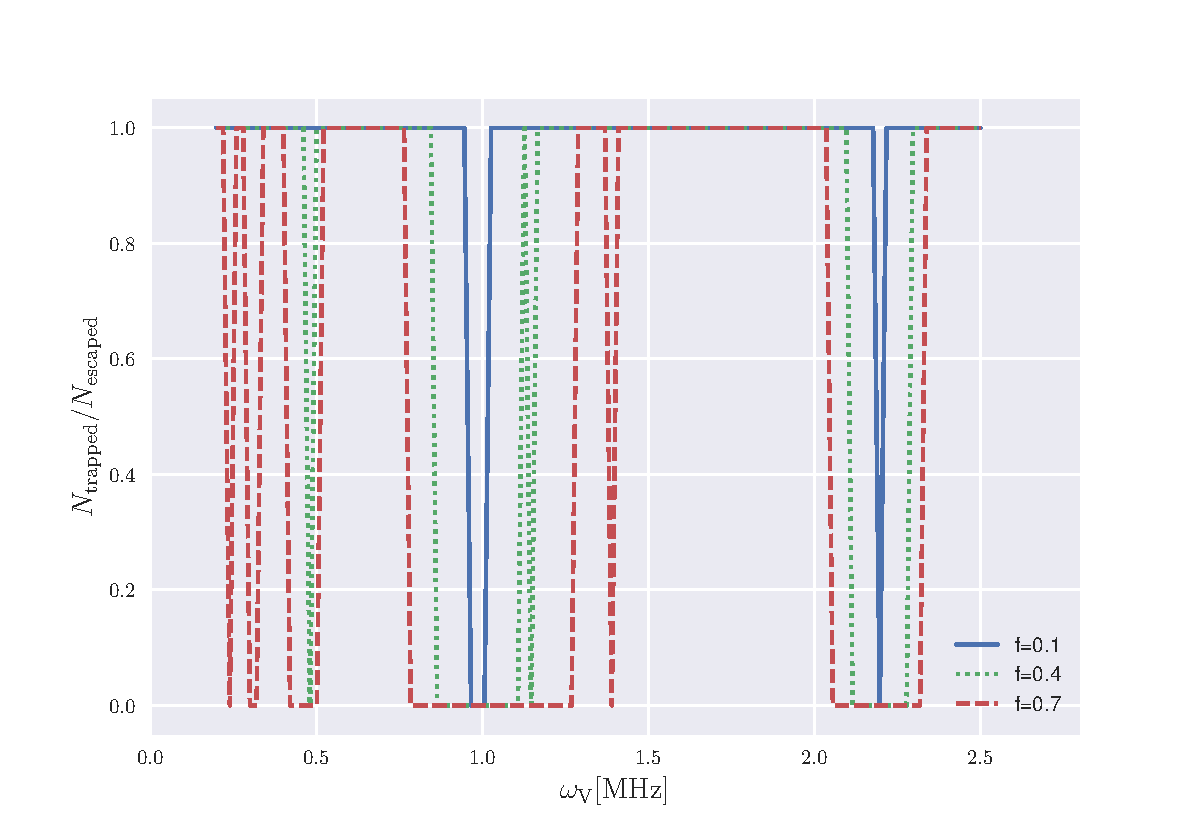
\includegraphics[width=1.\linewidth]{../figures/fraction_left_omega.pdf}
\caption{The fraction of the initial $100$ particles left after $500$ $\mu$s in the Penning trap with an oscillating $\bold{E}$-field over
the oscillation frequency. The simulations were run with three different amplitudes $f$. The angular frequencies of the analytical solution for the motion
of a single particle is marked by black dots. $\omega_{+} \approx 2.3$ MHz and $2\omega_{-} \approx 2.1$ MHz.}
\label{fig:fraction_noint}
\end{figure}

The fraction of particles left
in the trap after $500 \mu s$ as a function of frequency is shown in \autoref{fig:fraction_noint}.

The fraction of particles left in the trap is drastically reduced for some frequencies.
%revise: Actually, it quickly hits zero. Using this method for isolating particles will take some fine-tuning.
These correspond to the natural frequencies of the system.
Let us say a particle is in the left half of the trap as shown in \autoref{fig:penning} and travelling to the
left. If the field is now strong, the particle's velocity will increase. The magnetic field accelerates the
particle to turn and travel towards the right in the figure. Suppose the potential oscillations align with
the particle's motion. In that case, the potential is weak when the particle is in the left half travelling
towards the right and strong again when the particle is entering the right half. The potential will add
a substantially higher amount of energy to the particle than it detracts. Eventually, the particle will
move too fast for the magnetic field to confine it within the trap.

We see that the resonance frequencies are roughly halved. This corresponds to 'kicking' the particle only once per period or every second per period. This can explain why the low amplitude oscillations do not manage to kick out particles at lower frequencies. It is unable to provide enough energy for the particle to escape. It is also worth noting that the resolution is sharper for
the lower amplitude oscillations need to sync up better with the resonance frequency to deliver energy to the system.
Intuitively this makes much sense. The force is applied to the particles over a specific period. If the oscillations are not quite in
sync, the $\bold{E}$-field will decrease the kinetic energy of the particles for some part of this time, as it accelerates the particle in the
direction opposite of its motion. If the applied force is strong, the particle will still have a net gain in kinetic energy. If the applied force is
weak, this effect might stall the particles. The low amplitude oscillations give a better resolution because it is more dependent on syncing
 up with the natural frequency of the particles to provide a net gain in energy.

The angular frequencies of the analytical solution for the motion of a single particle \ref{eq:omega_pm} is $\omega_{+} \approx 2.30$ and $\omega_{-} \approx 1.05$. These are marked in the figure
as black dots. Notice that the highest resonance frequency appears dead in the centre of these.


%9.2
To see the effect of Coulomb interactions on the resonance of the trap
we perform simulations for the same duration and the same amount of particles
in the region around the resonance frequencies we
found. We chose to only simulate the amplitude $f = 0.1$ as this gave the sharpest troughs
in the former simulation.

\begin{figure}
\centering
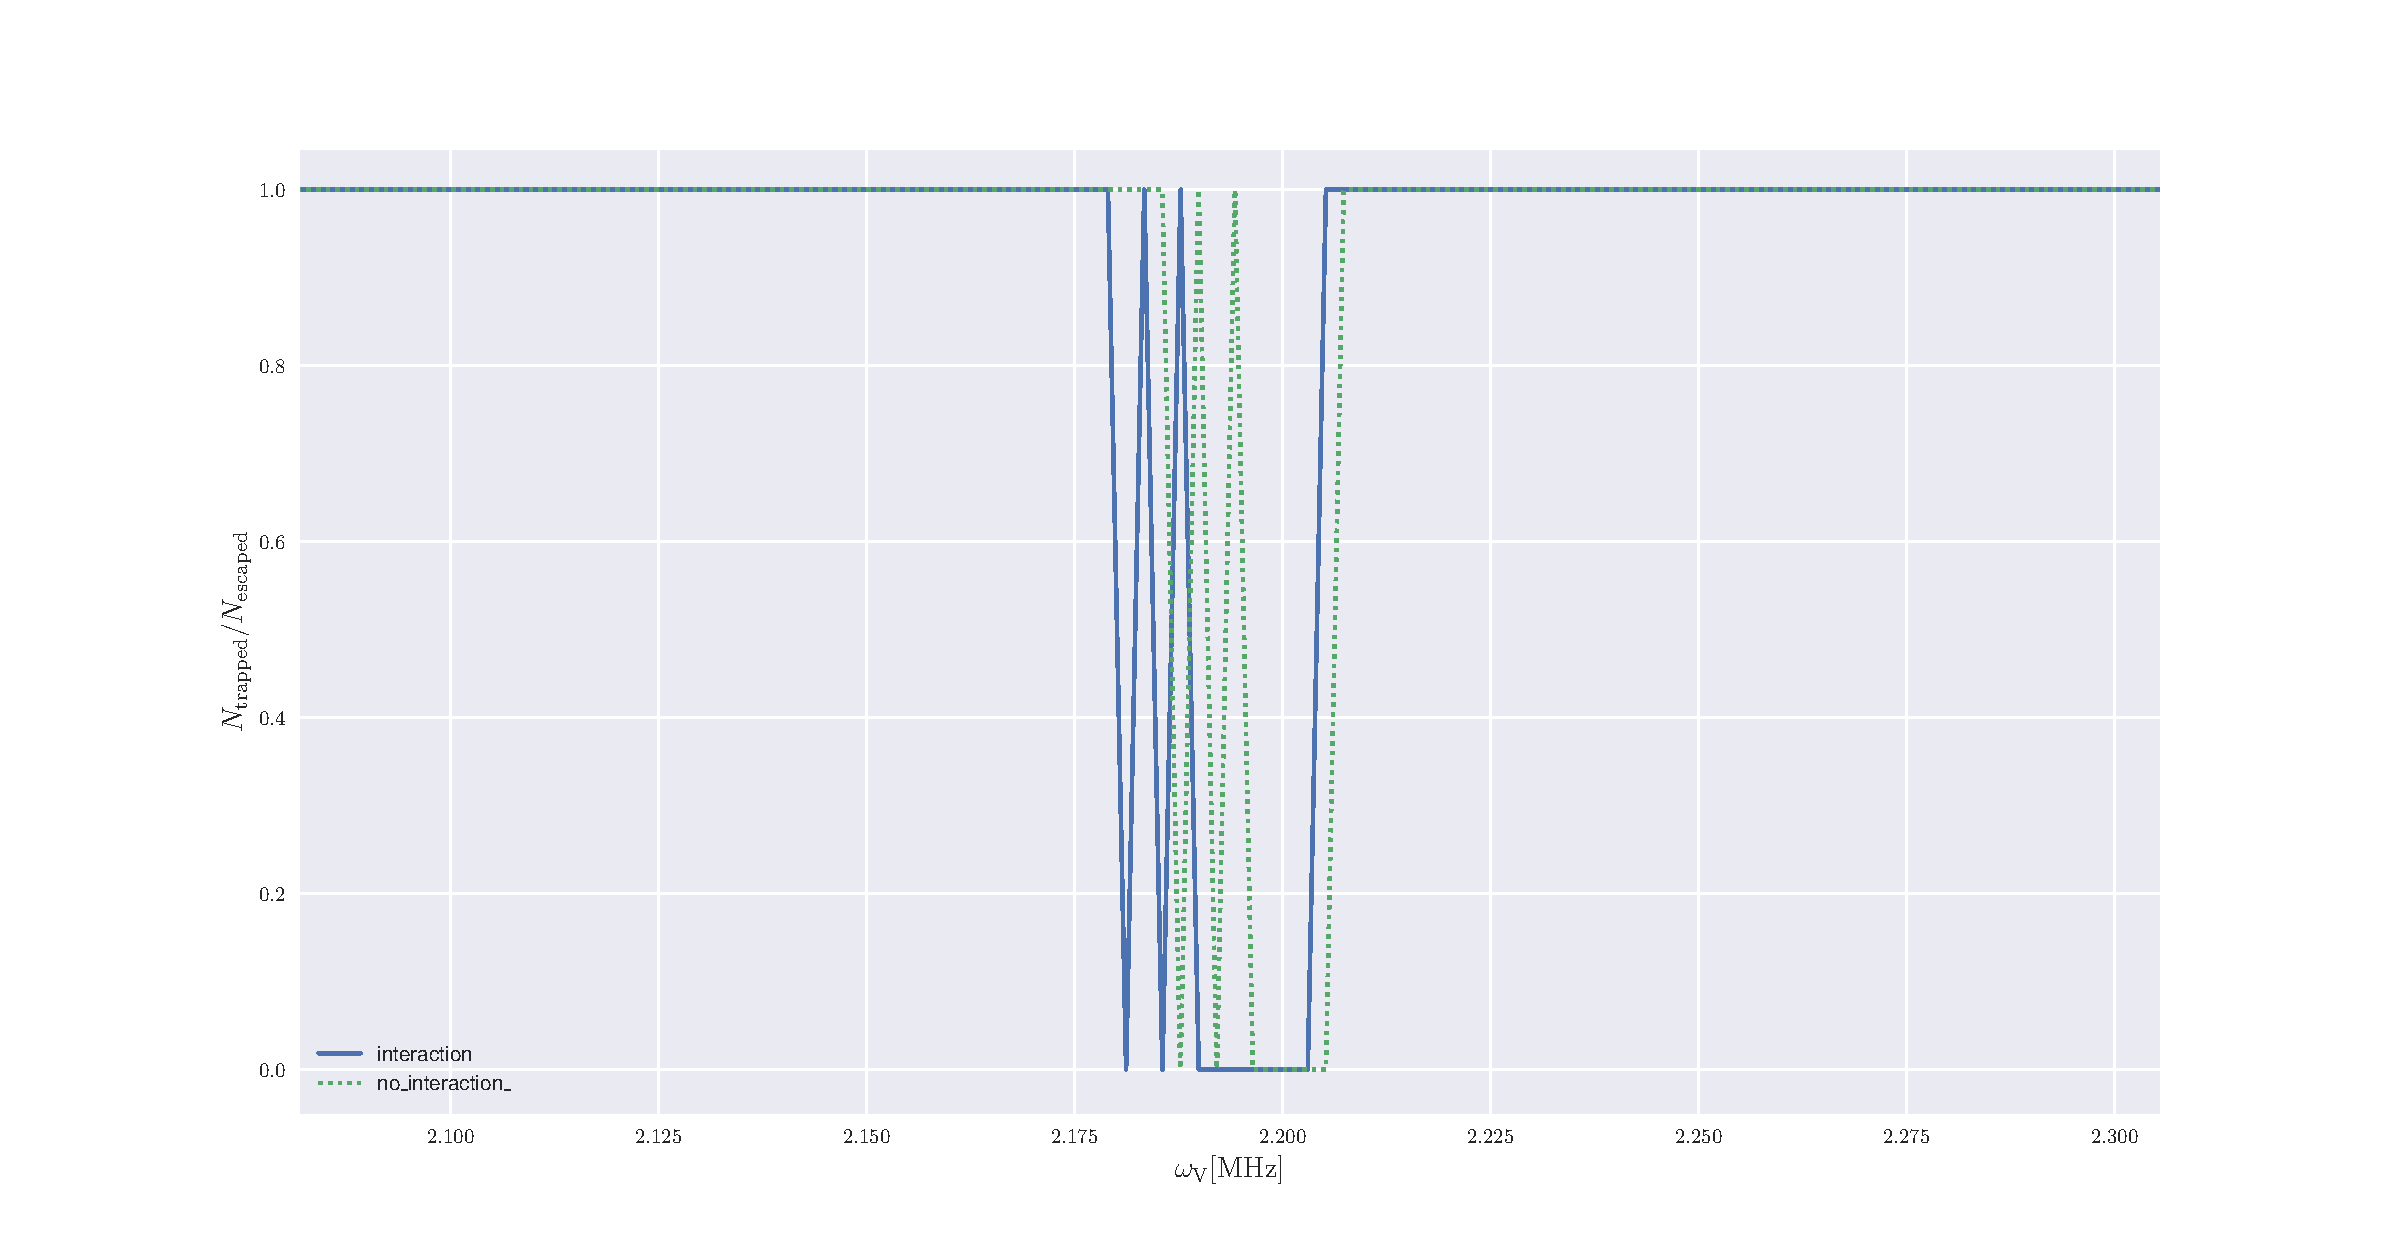
\includegraphics[width=1.\linewidth]{../figures/fraction_left_interaction.pdf}
\caption{Fraction of particles left of the initial $100$ particles, the blue line is for interacting particles, 
the green dotted line is for non-interacting particles. The perturbation amplitude is $f = 0.1$. }
\label{fig:fraction_int}
\end{figure}

The results are shown in \autoref{fig:fraction_int}.
Higher resolution shows that more frequencies are close together, not just one. This is
true both in the case of single particles, ignoring interactions and with many particles.
This might be due to the precessions of the particles in the $xy$-plane. Different frequencies might align
up with different 'subcircles', as seen in \autoref{fig:xy_plane}. It might also be the case that it will align
up with one such precession for the first kick and then shift by one for the next kick. This is plausible if the
particles have a steady time period for one orbit about the centre.
This is somewhat speculative. We need to find out if the orbits are steady, even in the case where we ignore
the interactions. Probably the particle periods are only partially constant.

In comparing the interacting particles to the non-interacting particles, we notice a slight
shift in all the resonance frequencies. It appears to be constant, but this might be
an effect of too low resolution. Alas, we do not know.

A possible explanation of why the resonance frequencies are lower in the
case of interacting particles might be because the particles can distribute the energy among
themselves. Let us imagine one particle is being kicked, pushing the next particle 'in line', which again
pushes the next particle and so forth. This highly idealized illustration can explain how a
compression wave propagates through the particles in the trap. If some of the energy is bound to
compression waves, we expect that the mean velocity of the particles is somewhat slower, making the
orbital period longer. This is one reasonable explanation which we do not intend to verify.
